\documentclass[11pt,a4paper]{article}
% Working-paper version converted from the Word manuscript.
% Compile with pdfLaTeX + BibTeX (Overleaf's standard PDFLaTeX setting).
\usepackage[T1]{fontenc}
\usepackage[utf8]{inputenc}
\usepackage{newtxtext,newtxmath}
\usepackage[margin=27mm]{geometry}
\usepackage{microtype}
\usepackage{setspace}
\usepackage{amsmath,bm}
\usepackage{graphicx}
\usepackage{booktabs}
\usepackage{multirow}
\usepackage{tikz}
\usetikzlibrary{arrows.meta}
\usepackage{caption}
\usepackage{subcaption}
\usepackage[section]{placeins}
\usepackage[round,authoryear]{natbib}
\usepackage[hidelinks]{hyperref}
\setstretch{1.12}
\setlength{\parindent}{1.4em}
\setlength{\parskip}{0pt}
\captionsetup{font=small,labelfont=bf}
\captionsetup[sub]{font=small,labelformat=parens}
\graphicspath{{figures/}}
\title{Stochastic Bimodal Day-to-Day Dynamic Traffic Assignment}
\author{}
\date{\textit{Working manuscript}}
\begin{document}
\maketitle
\vspace{-1.8em}

\noindent\textbf{Keywords:} Day-to-day dynamic traffic assignment; multimodal transport; stochastic user equilibrium; bounded choice model; proportion-based adjustment.
\vspace{1em}


\section{Introduction}\label{sec:introduction}

Day-to-day dynamic traffic assignment describes how travellers adjust their travel decisions over successive days and how the resulting traffic patterns evolve towards equilibrium. Since \citet{smith1984}, this topic has provided an important link between individual route adjustment, equilibrium analysis and transport-network performance.

Existing models differ in several respects, including whether adjustment is deterministic or stochastic, whether time is treated as continuous or discrete, whether travellers follow deterministic, probabilistic or boundedly rational choice rules, and whether the state is represented by link or path flows \citep{cantarella2016det,cantarella2016stoch,zhou2020}. Much of this literature concerns single-mode networks, particularly private-car traffic.

In a multimodal network, travellers may change both their route within a mode and their transport mode. This creates an additional challenge: modal demand may change from day to day, so a route-adjustment formulation should remain consistent with the evolving distribution of demand across modes. Earlier two-mode studies provide useful foundations but often adopt simplified within-mode route representations \citep{cantarella2015,guo2018}.

This working manuscript examines stochastic day-to-day dynamics in a bimodal car--bus network with multiple routes available within each mode. It considers conventional logit stochastic user equilibrium (SUE) and stochastic user equilibrium with a bounded choice model (BCM), following \citet{watling2018}.

The central modelling idea is to represent within-mode route adjustment through path-choice proportions while allowing modal demands to change. This representation provides a basis for examining flow consistency across the two levels of choice. Detailed adjustments and analytical derivations are outside the scope of this working version.

The numerical illustrations focus on three aspects: the evolution of mode and path flows under the logit model; the effects of different BCM thresholds on convergence and choice-set composition; and sensitivity of the final numerical solution to different initial flow patterns.

Two cost representations, referred to below as Type I (local) and Type II (global), are also compared numerically. The discussion focuses on the patterns illustrated by the reported results.

The following sections present the modelling framework, outline the numerical method, and discuss the illustrative results and their limitations.


\section{Modelling framework}\label{sec:framework}


\subsection{Network and travel costs}

Consider a bimodal transport network $G=(N,A)$, with node set $N$, link set $A$ and travel modes $M=\{\mathrm{car},\mathrm{bus}\}$. For each mode $m$, $A^m$ denotes its link set. The illustrative setting assumes separated car and bus links ($A^{\mathrm{car}}\cap A^{\mathrm{bus}}=\varnothing$), as could occur with dedicated bus infrastructure. Let $W$ denote the origin--destination pairs. For each pair $w$, total demand $D^w$ is fixed and $P^{wm}$ is the predefined path set for mode $m$. The following conventional functions specify flow-dependent link costs for car and bus:

\begin{equation}
c_a^{\mathrm{car}}=t_{a,0}^{\mathrm{car}}\!\left(1+\alpha^{\mathrm{car}}\!\left(\frac{v_a^{\mathrm{car}}}{C_a^{\mathrm{car}}}\right)^{\beta^{\mathrm{car}}}\right),\quad \forall a\in A^{\mathrm{car}}
\label{eq:car-cost}
\end{equation}

\begin{equation}
c_a^{\mathrm{bus}}=t_{a,0}^{\mathrm{bus}}+\alpha^{\mathrm{bus}}\!\left(\frac{v_a^{\mathrm{bus}}}{C_a^{\mathrm{bus}}}\right)^{\beta^{\mathrm{bus}}},\quad \forall a\in A^{\mathrm{bus}}
\label{eq:bus-cost}
\end{equation}

where link flow is determined by the path--link incidence relationship:

\begin{equation}
v_a^m=\sum_{w\in W}\sum_{r\in P^{wm}}\Delta_a^{wr}\,f_r^{wm},\quad \forall m\in M,\ a\in A^m
\label{eq:link-flow}
\end{equation}

In Eqs.~\eqref{eq:car-cost} and \eqref{eq:bus-cost}, $t_{a,0}^m$ denotes the baseline link travel cost, $C_a^m$ the link capacity, $v_a^m$ the link flow, and $\alpha^m$ and $\beta^m$ calibrated parameters. Equation~\eqref{eq:car-cost} uses a conventional Bureau of Public Roads (BPR)-type form. For bus links, the baseline cost can incorporate waiting and in-vehicle time, while the second term represents an additional flow-dependent cost. Equation~\eqref{eq:link-flow} links path flows to link flows using the path--link incidence indicators.

The cost of a path is the sum of the costs of its constituent links:

\begin{equation}
c_r^{wm}=\sum_{a\in A^m}\Delta_a^{wr}\,c_a^m,\quad \forall w\in W,\ r\in P^{wm},\ m\in M
\label{eq:path-cost}
\end{equation}

The illustrative cost specification involves two simplifying assumptions.

First, the bus cost function does not explicitly model the common-lines problem or bus frequency in the waiting-time calculation. This gives a tractable flow-dependent cost specification; a frequency-based transit formulation could have different mathematical properties \citep{szeto2014,jiang2016}.

Second, path costs are assumed to be link-additive. This is convenient for the present numerical study but does not cover every cost structure, including some route-specific fares or charges \citep{han2004}. Both assumptions limit the direct applicability of the illustrative network model.

Figure~\ref{fig:network} presents the example network, comprising one origin--destination pair, four car paths and two bus paths. Each path is represented by a separate link for simplicity. The network and parameter values are used in the numerical illustrations in Section~\ref{sec:numerical}.

\begin{figure}[tbp]
\centering
\begin{minipage}[c]{0.42\linewidth}
\centering
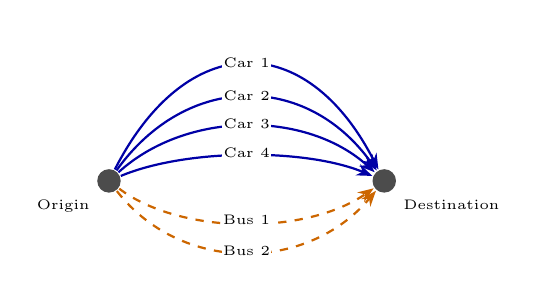
\begin{tikzpicture}[x=0.76cm,y=0.69cm,>=Stealth,thick]
  \node[circle,fill=black!70,inner sep=3pt,label={[font=\tiny]below left:Origin}] (o) at (0,0) {};
  \node[circle,fill=black!70,inner sep=3pt,label={[font=\tiny]below right:Destination}] (d) at (4.6,0) {};
  \foreach \y/\name in {2.8/1,2.0/2,1.3/3,0.6/4}{
    \draw[-{Stealth[length=2mm]},blue!65!black] (o) .. controls (1.3,\y) and (3.3,\y) .. (d);
    \node[fill=white,inner sep=0.5pt,font=\tiny] at (2.3,{0.75*\y+0.07}) {Car \name};
  }
  \draw[-{Stealth[length=2mm]},dashed,orange!80!black] (o) .. controls (1.2,-1.0) and (3.3,-1.0) .. (d);
  \draw[-{Stealth[length=2mm]},dashed,orange!80!black] (o) .. controls (1.2,-1.7) and (3.3,-1.7) .. (d);
  \node[fill=white,inner sep=0.5pt,font=\tiny] at (2.3,-0.72) {Bus 1};
  \node[fill=white,inner sep=0.5pt,font=\tiny] at (2.3,-1.28) {Bus 2};
\end{tikzpicture}
\end{minipage}\hfill
\begin{minipage}[c]{0.55\linewidth}
\centering\footnotesize
\begin{tabular}{lrrrr}
\toprule
Path & $t^m_{a,0}$ & $C_a^m$ & $\alpha^m$ & $\beta^m$\\
\midrule
Car 1 & 15 & 60 & 0.15 & 4\\
Car 2 & 8 & 40 & 0.15 & 4\\
Car 3 & 12 & 50 & 0.15 & 4\\
Car 4 & 9 & 50 & 0.15 & 4\\
Bus 1 & 10 & 100 & 1.00 & 2\\
Bus 2 & 12 & 50 & 1.00 & 2\\
\bottomrule
\end{tabular}
\end{minipage}
\caption{Illustrative bimodal network and input parameters. For simplicity, each path is represented by one link.}
\label{fig:network}
\end{figure}


\subsection{Mode choice}

For a given set of path costs, mode-level composite utility is specified by the logsum expression:

\begin{equation}
u^{wm}=\frac{1}{\theta^{wm}}\ln\!\left(\sum_{r\in P^{wm}}\exp\!\left(-\theta^{wm}c_r^{wm}\right)\right),\quad \forall m\in M,\ w\in W
\label{eq:logsum}
\end{equation}

The expression aggregates the path costs within a mode, with the route-choice scale parameter controlling sensitivity to cost. Mode-specific demand is then obtained from the logit mode-choice relationship:

\begin{equation}
d^{wm}=D^w\,\frac{\exp\!\left(\theta^w u^{wm}\right)}{\displaystyle\sum_{k\in M}\exp\!\left(\theta^w u^{wk}\right)},\quad \forall m\in M,\ w\in W
\label{eq:mode-demand}
\end{equation}

Here total demand for each origin--destination pair is fixed, while the allocation of demand between car and bus is endogenous. The mode-choice scale parameter determines the responsiveness of modal demand to the composite utilities.


\subsection{Within-mode route choice}


\subsubsection{Logit stochastic user equilibrium}

With a predefined path set for each mode and origin--destination pair, the conventional logit model assigns the following path-choice proportions:

\begin{equation}
\alpha_p^{wm}=\frac{\exp\!\left(-\theta^{wm}c_p^{wm}\right)}{\displaystyle\sum_{k\in P^{wm}}\exp\!\left(-\theta^{wm}c_k^{wm}\right)},\quad \forall m\in M,\ w\in W,\ p\in P^{wm}
\label{eq:logit-route}
\end{equation}

The specification uses a predefined set of feasible paths; path generation is outside the scope of this working version. Given the mode demand and the within-mode path-choice proportion, path flow follows from:

\begin{equation}
f_p^{wm}=d^{wm}\,\alpha_p^{wm},\quad \forall m\in M,\ w\in W,\ p\in P^{wm}
\label{eq:flow-allocation}
\end{equation}

The same set of travel modes is not required for every origin--destination pair. If only one mode is available, the mode-choice step can be omitted for that pair.

The relation between modal demand, route-choice proportions and path flows makes the within-mode flow accounting explicit.


\subsubsection{Stochastic user equilibrium with a bounded choice model}

The bounded choice model (BCM) restricts the routes considered by travellers according to a cost threshold relative to the minimum-cost alternative. A route outside that bounded choice set has zero choice probability. The route-choice expression retained here follows the formulation of \citet{watling2018}:

\begin{equation}
\bar{\alpha}_p^{wm}=\frac{
\left\{\exp\!\left[-\theta^{wm}\!\left(c_p^{wm}-\min_{r\in P^{wm}}\{c_r^{wm}\}-\delta^{wm}\right)\right]-1\right\}_+
}{
\displaystyle\sum_{q\in P^{wm}}\left\{\exp\!\left[-\theta^{wm}\!\left(c_q^{wm}-\min_{r\in P^{wm}}\{c_r^{wm}\}-\delta^{wm}\right)\right]-1\right\}_+
},
\label{eq:bcm-route}
\end{equation}

Here $\{x\}_+=\max\{0,x\}$ and $\delta^{wm}$ is the threshold for mode $m$ and OD pair $w$. The threshold is allowed to vary by mode and origin--destination pair. Compared with conventional logit SUE, the BCM can exclude sufficiently unattractive routes from consideration. The resulting path flows are calculated using the same flow-allocation relationship given above.


\section{Day-to-day adjustment framework}\label{sec:adjustment}


\subsection{Bimodal stochastic dynamics}

The model considers successive adjustments in modal demands and in the proportions choosing paths within each mode. The state therefore includes both modal-demand variables and within-mode path-choice proportions, rather than treating all modal path flows as independently fixed-demand variables.

A stationary state of the adjustment system may be represented by the following generic equilibrium condition, where the adjustment mapping vanishes:

\begin{equation}
\bm\Phi\!\left(\mathbf d(t),\bm\alpha(t)\right)=\mathbf 0
\label{eq:stationary}
\end{equation}


\subsection{Flow conservation and choice hierarchy}

The key distinction from a single-mode fixed-demand formulation is that total origin--destination demand is conserved while the demand assigned to each mode may change. For that reason, a route-adjustment mechanism expressed in terms of proportions is considered alongside a separate modal-demand adjustment.

A proportion-based description retains the distinction between choosing a mode and choosing a route conditional on that mode. It also avoids interpreting the conservation of route flows within one mode as conservation of that mode's total demand when travellers switch between modes.

Both the logit SUE and the BCM specifications are considered within this framework. In the latter, the bounded path-choice set may change as congestion and path costs evolve; the numerical experiments below illustrate this behaviour.

The treatment here emphasises the structure of the adjustment process and the behavioural distinction between the two route-choice specifications.


\subsection{Local and global equilibrium-cost representations}

For numerical interpretation of the BCM dynamics, the study considers two path-cost representations: Type I (local), associated with routes in the bounded choice set, and Type II (global), which is evaluated across the full path set. Their numerical behaviour is the focus of the comparison below.

These two quantities need not take the same values during the adjustment process. Their numerical behaviour is compared in Figure~\ref{fig:costs} for different choice-set thresholds.

In the reported experiments, equality of the Type I costs is observed among paths in the bounded choice set, whereas the Type II costs approach a common value across the illustrated paths. These are observations from the examples rather than a general analytical result established in this document.

This comparison is relevant to the interpretation of the numerical procedure, particularly when a route enters or leaves the bounded set during adjustment.


\section{Computational procedure (overview)}\label{sec:algorithm}

The numerical procedure alternates between adjustments to modal demands, adjustments to within-mode path-choice proportions, and updates of link, path and mode costs. Iteration continues until the reported convergence-gap criterion is satisfied. This overview describes the computational sequence without specifying the individual pairwise updates.


\section{Numerical illustrations}\label{sec:numerical}

All experiments use the illustrative network in Figure~\ref{fig:network}. The initial car-path flows, ordered by path number, are 20, 60, 80 and 40; the initial bus-path flows are 20 and 30. The mode-choice scale parameter is 0.1, and the reported step sizes for mode-demand and path-proportion adjustment are 0.1 and 0.001, respectively. Unless otherwise stated, the stopping criterion is a convergence gap below $10^{-4}$. The examples compare the baseline logit dynamics, the bounded-choice dynamics and sensitivity to initial conditions.


\subsection{Evolution under the logit SUE model}

Figure~\ref{fig:sue} illustrates the day-to-day evolution of the numerical gap, modal demands and path flows. The gap decreases smoothly towards the stopping threshold in this example (Figure~\ref{fig:sue}a). Car demand declines while bus demand increases before both approach steady values (Figure~\ref{fig:sue}b). The bus-path flows evolve smoothly (Figure~\ref{fig:sue}c), whereas some car-path flows show non-monotonic trajectories even though the overall gap declines (Figure~\ref{fig:sue}d).

\begin{figure}[tbp]
\centering
\begin{subfigure}[t]{0.48\linewidth}\centering
  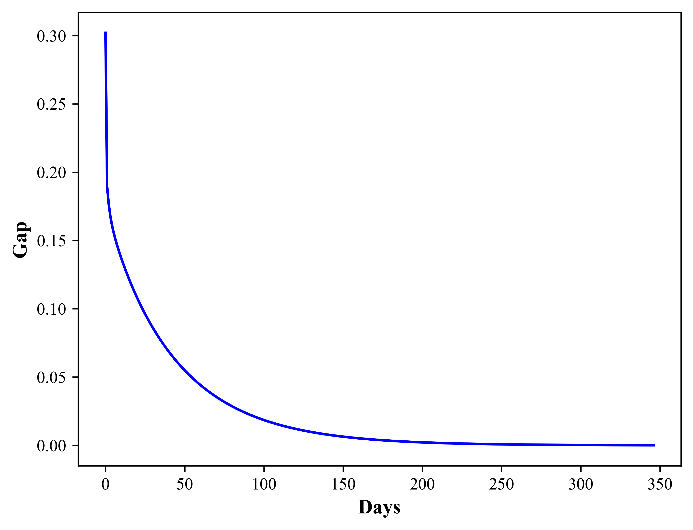
\includegraphics[width=\linewidth]{sue_gap.png}
  \caption{Convergence gap}\end{subfigure}\hfill
\begin{subfigure}[t]{0.48\linewidth}\centering
  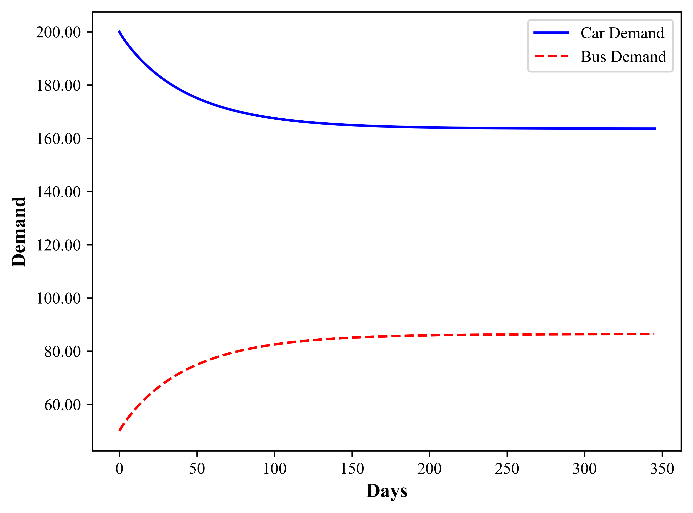
\includegraphics[width=\linewidth]{sue_mode.png}
  \caption{Modal demand}\end{subfigure}\\[0.6em]
\begin{subfigure}[t]{0.48\linewidth}\centering
  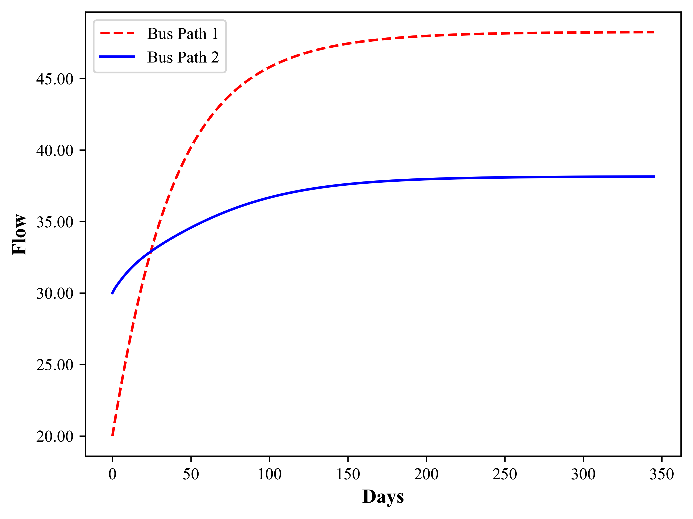
\includegraphics[width=\linewidth]{sue_bus.png}
  \caption{Bus-path flows}\end{subfigure}\hfill
\begin{subfigure}[t]{0.48\linewidth}\centering
  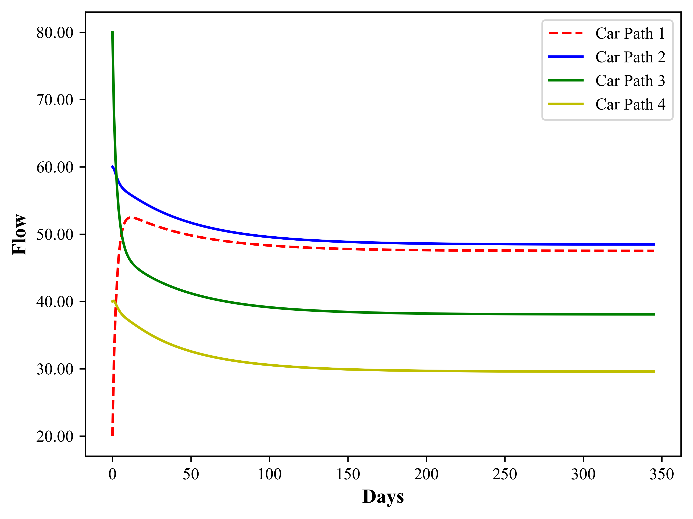
\includegraphics[width=\linewidth]{sue_car.png}
  \caption{Car-path flows}\end{subfigure}
\caption{Evolution of the convergence gap, modal demands and path flows under logit SUE.}
\label{fig:sue}
\end{figure}


\subsection{Sensitivity to the bounded-choice threshold}

Figure~\ref{fig:bcm-gap} compares the BCM results for two thresholds, $\delta^{wm}=5$ and $\delta^{wm}=1$. With the larger threshold, additional car paths enter the bounded choice set early in the adjustment, and the convergence-gap curve is relatively smooth. With the smaller threshold, the choice set changes at later iterations and the gap curve exhibits several distinct changes in slope. Table~\ref{tab:choice-sets} records the sequence of car-path choice sets in each case.

\begin{figure}[tbp]
\centering
\begin{subfigure}[t]{0.48\linewidth}\centering
  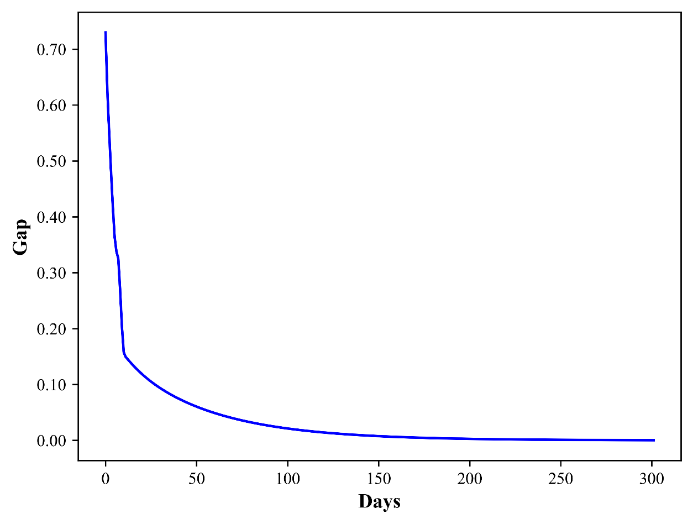
\includegraphics[width=\linewidth]{bcm_gap_5.png}
  \caption{$\delta^{wm}=5$}\end{subfigure}\hfill
\begin{subfigure}[t]{0.48\linewidth}\centering
  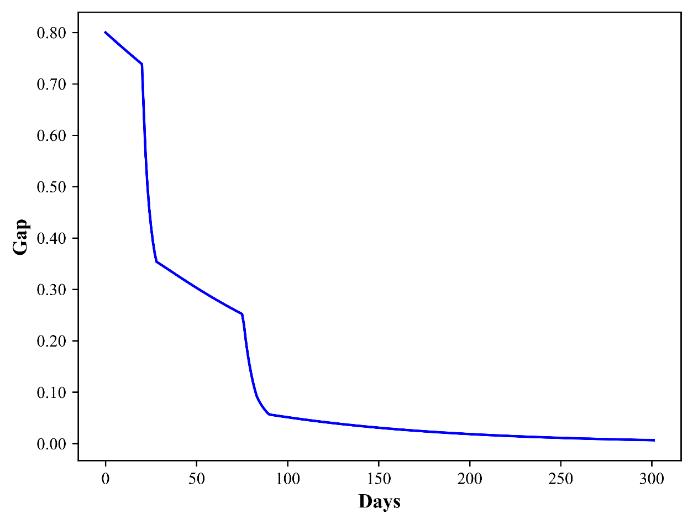
\includegraphics[width=\linewidth]{bcm_gap_1.png}
  \caption{$\delta^{wm}=1$}\end{subfigure}
\caption{BCM convergence gaps for the two bounded-choice thresholds.}
\label{fig:bcm-gap}
\end{figure}
\FloatBarrier

\begin{center}
\captionsetup{type=table}
\centering
\caption{Evolution of the car-path bounded choice set for the two thresholds.}
\label{tab:choice-sets}
\small
\begin{tabular}{llccc}
\toprule
Threshold & Measure & Period 1 & Period 2 & Period 3\\
\midrule
\multirow{2}{*}{$\delta^{wm}=5$} & Days & 0--2 & 3--7 & 8--300\\
 & Bounded choice set & $\{2,4\}$ & $\{1,2,4\}$ & $\{1,2,3,4\}$\\
\addlinespace[3pt]
\multirow{2}{*}{$\delta^{wm}=1$} & Days & 0--20 & 21--75 & 76--300\\
 & Bounded choice set & $\{4\}$ & $\{2,4\}$ & $\{2,3,4\}$\\
\bottomrule
\end{tabular}
\end{center}

Figure~\ref{fig:costs} compares the two equilibrium-cost representations for the same thresholds. For $\delta^{wm}=5$, the plotted car-path costs move towards a common level in both representations. For $\delta^{wm}=1$, the Type I curves are closely aligned only among routes included in the bounded set, while the Type II curves move towards a common level across the four plotted car paths. The changes in these trajectories coincide with changes in the bounded choice set. The figures illustrate the distinction between the cost measures but do not, by themselves, establish a convergence theorem.

\begin{figure}[tbp]
\centering
\begin{subfigure}[t]{0.48\linewidth}\centering
  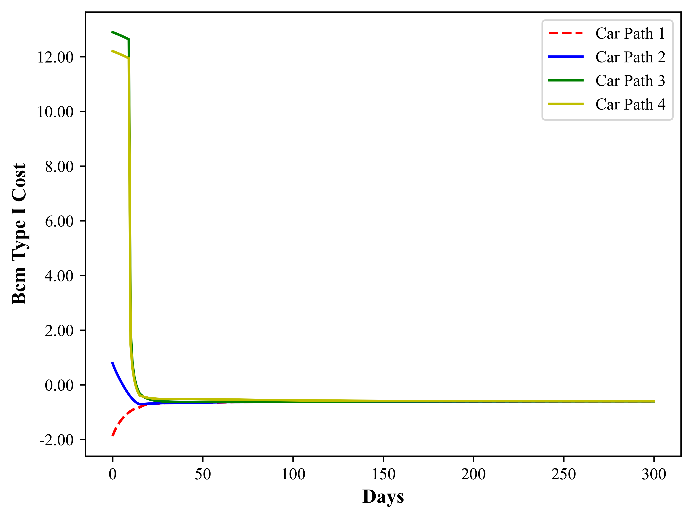
\includegraphics[width=\linewidth]{bcm_local_5.png}
  \caption{Type I, $\delta^{wm}=5$}\end{subfigure}\hfill
\begin{subfigure}[t]{0.48\linewidth}\centering
  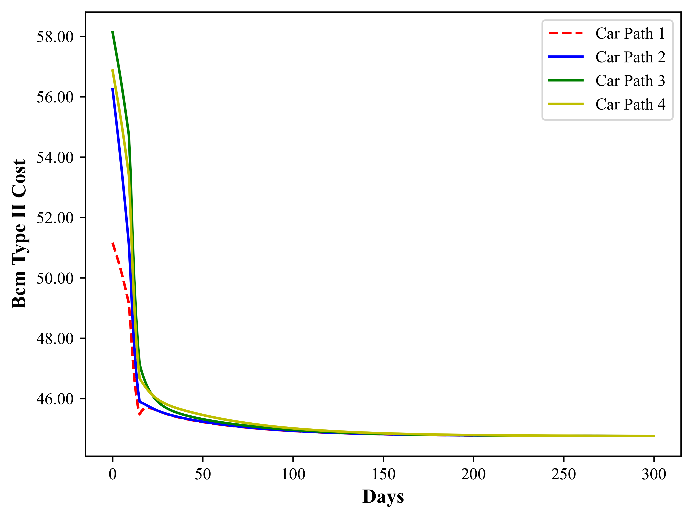
\includegraphics[width=\linewidth]{bcm_global_5.png}
  \caption{Type II, $\delta^{wm}=5$}\end{subfigure}\\[0.6em]
\begin{subfigure}[t]{0.48\linewidth}\centering
  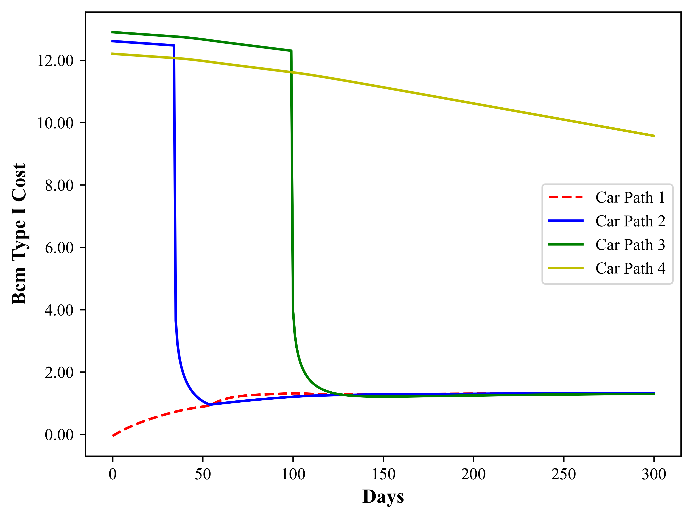
\includegraphics[width=\linewidth]{bcm_local_1.png}
  \caption{Type I, $\delta^{wm}=1$}\end{subfigure}\hfill
\begin{subfigure}[t]{0.48\linewidth}\centering
  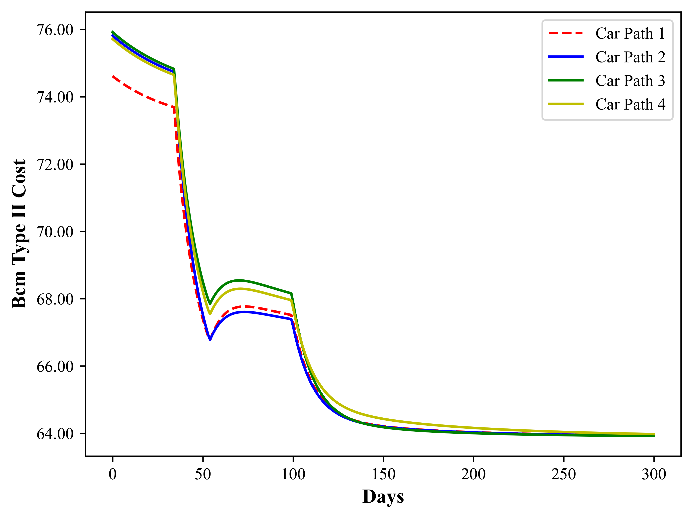
\includegraphics[width=\linewidth]{bcm_global_1.png}
  \caption{Type II, $\delta^{wm}=1$}\end{subfigure}
\caption{Evolution of Type I (local) and Type II (global) costs for the two thresholds.}
\label{fig:costs}
\end{figure}
\FloatBarrier


\subsection{Sensitivity to initial flow allocations}

A further numerical experiment uses 1,000 randomly generated initial flow allocations with fixed total demand and a tighter convergence-gap tolerance of $10^{-6}$. Table~\ref{tab:stability} reports the mean and standard deviation of the number of iterations (days) required to meet this criterion, together with the maximum across-path standard deviation of the final path flows. For the tested cases, all runs met the stopping criterion and yielded closely aligned final flows. This provides numerical evidence of robustness to initialisation on the illustrative network; it is not a proof of global stability or uniqueness.

\begin{table}[tbp]
\centering
\caption{Convergence and final-flow variation over 1,000 initialisations.}
\label{tab:stability}
\small
\begin{tabular}{llccc}
\toprule
 & & SUE & BCM ($\delta^{wm}=5$) & BCM ($\delta^{wm}=1$)\\
\midrule
\multirow{2}{*}{Days to convergence} & Mean & 528 & 549 & 1208\\
 & Standard deviation & 51 & 50 & 84\\
\addlinespace[2pt]
\multicolumn{2}{l}{Max. standard deviation of final path flows} & $1.20\times10^{-4}$ & $1.20\times10^{-4}$ & $4.78\times10^{-7}$\\
\bottomrule
\end{tabular}
\vspace{0.3em}
\parbox{0.94\linewidth}{\footnotesize\emph{Note:} Convergence is defined by a gap below $10^{-6}$.}
\end{table}


\section{Discussion and concluding remarks}\label{sec:conclusion}

The illustrative results demonstrate how stochastic bimodal day-to-day adjustment can be examined with explicit within-mode route choice and changing modal demand. In the examples, the logit dynamics yield smooth decreases in the convergence gap; the BCM threshold affects both the evolving choice set and the shape of the convergence trajectory; and different initial allocations lead to closely aligned numerical endpoints. The Type I and Type II cost plots additionally highlight the importance of distinguishing between the bounded and full path sets. These conclusions are limited to the reported numerical settings. A general stability result, detailed update equations and larger-network evidence are not established in this working manuscript.

\section*{Acknowledgement}

This work was partially supported by Independent Research Fund Denmark (Grant 2035-00111B).

\nocite{*}
\bibliographystyle{plainnat}
\bibliography{references}
\end{document}
